\documentclass[tikz,convert={outext=.png}]{standalone}
\begin{document}
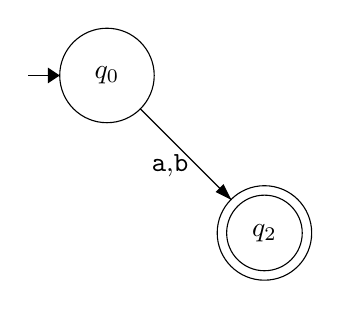
\begin{tikzpicture}[scale=0.2]
\tikzstyle{every node}+=[inner sep=0pt]
\draw [black] (-5,0) -- (-3,0);
\fill [black] (-3,0) -- (-3.75,-.5) -- (-3.75,.5);
\draw [black] (0,0) circle (3);
\draw (0,0) node {$q_0$};

\draw (4, -5) node [below] {{\tt a},{\tt b}};
\draw [black] (2.1,-2.1) -- (7.9,-7.9);
\fill [black] (7.9,-7.9) -- (6.9,-7.4) -- (7.4,-6.9);
\draw [black] (10,-10) circle (3);
\draw [black] (10,-10) circle (2.4);
\draw (10,-10) node {$q_2$};
\end{tikzpicture}
\end{document}
